% Implementation report.
%
% This is NOT a copy of README.md. The README is the specification; this reports
% what implementing it found -- the resolutions of underspecified points, the
% measurements, and the places where a claim had to be weakened or corrected.
%
% Build:  latexmk -pdf main.tex     (or: pdflatex, bibtex, pdflatex x2)
% Figures come from scripts/make_figures.py and are expected in ../figures/.

\documentclass[11pt,a4paper]{article}

% lmodern before fontenc: T1 with the default Computer Modern selects bitmap
% fonts, and microtype's font expansion below requires scalable ones.
\usepackage{lmodern}
\usepackage[T1]{fontenc}
\usepackage[utf8]{inputenc}
\usepackage[british]{babel}
\usepackage{amsmath,amssymb,amsthm}
\usepackage{booktabs}
\usepackage{graphicx}
\usepackage{microtype}
\usepackage[margin=2.5cm]{geometry}
\usepackage[hidelinks]{hyperref}
\usepackage{listings}
\usepackage{xcolor}

\theoremstyle{plain}
\newtheorem{proposition}{Proposition}
\theoremstyle{remark}
\newtheorem{finding}{Finding}

\newcommand{\addendum}[1]{\textsf{G#1}}
\newcommand{\code}[1]{\texttt{\small #1}}

\lstset{
  basicstyle=\ttfamily\footnotesize,
  breaklines=true,
  frame=single,
  rulecolor=\color{gray!40},
  columns=fullflexible,
}

\title{Numerical Stability and Perturbation Behaviour in\\
       TF-IDF-Based Similarity Systems\\[0.4em]
       \large An implementation report}
\author{Matthew Maksymilian Miezaniec}
\date{}

\begin{document}
\maketitle

\begin{abstract}
This report accompanies the specification in \code{README.md}. It records what
building the system established that the specification did not state, and what
had to be corrected. Three results are structural rather than incidental. First,
the numerical noise floor is roughly six orders of magnitude below the smallest
observed score separation, so floating-point error cannot reorder two
distinctly-scored documents; every ranking instability in the unperturbed
pipeline arises from \emph{exact} ties, and therefore from the tie-break.
Second, the tolerance $\tau$ admits no single principled value, but it does admit
a derived \emph{band} across which the reported tie structure is provably
invariant. Third, a fine near-tie cannot be manufactured by editing document
text, because term-frequency normalisation makes a single-token edit a relative
perturbation of order $1/L$; the case study of \S7.4 must therefore identify a
near-tie rather than construct one. Twenty-three addenda are recorded in
\code{docs/spec\_addenda.md}; this report summarises those that change what may
be claimed.
\end{abstract}

\section{Two implementations, one definition of correctness}

The system exists twice: a pure-Python reference and an optimised C++20 core.
The relationship between them is the central architectural commitment.

The \textbf{Python reference is normative}. It defines correctness, has no
compiled dependency, and every published number is defined by what it produces.
The \textbf{C++ core is an optimisation} required to be bit-identical, which the
test suite enforces by comparing raw bit patterns rather than tolerances. A
tolerance would silently admit precisely the divergence under study.

Bit-identity is asserted across four reduction policies, two scoring kernels
(term-at-a-time and document-at-a-time) and three ranking operators. For a
ranking the claim is \emph{permutation identity}, which holds given four
separately-testable conditions: the sort key is injective, its inputs are
identical, the comparison relation is the same in both languages, and the build
is not fast-math.

\section{Removing floating point rather than handling it}

\subsection{The logarithm}\label{sec:log}

\code{math.log} is not correctly rounded, and \addendum{13} records the
consequence: it differs from the correctly-rounded value in $15.16\%$ of IDF
entries, and UCRT, glibc and Apple libm disagree with one another. Left alone,
Linux and Windows produce different weights, norms, scores and rankings, and the
reproducibility claim is simply false.

IDF is therefore computed once in Python via \code{decimal.Decimal.ln()} at
60~digits and rounded once to binary64. The C++ core never sees a logarithm; it
receives IDF as data. What remains is $+$, $-$, $\times$, $\div$ and $\sqrt{\ }$,
which IEEE-754 requires to be correctly rounded~\cite{ieee754-2019}, so every
conforming platform must agree.

\subsection{The tie-break}

The same move is applied to ordering. Tie-break attributes are rank-encoded to
dense \code{int32} once per corpus, with direction and missing-value placement
baked into the rank rather than applied per comparison. Floating point is thereby
removed from the tie-break \emph{entirely} --- not by being careful with it, but
by there being none left --- and NaN cannot enter through the tie-break at all,
as a type-level guarantee.

\section{The measured noise floor, and the derivation of \texorpdfstring{$\tau$}{tau}}

\S7.1 asks that $\tau$ ``exceed floating-point noise while remaining small
relative to typical score separations''. That is a two-sided qualitative
constraint: it defines an interval, not a value, and gives no procedure. Deriving
a single number from it would manufacture precision the specification does not
contain.

\subsection{The lower endpoint}

$\tau$'s job is to decide whether $|s_i - s_j| \le \tau$ is evidence of a real
difference. The quantity to bound is therefore the error in a \emph{margin}, not
in a score. If each score carries error at most $\eta$, the margin carries at
most $2\eta$ and both signs are attainable, so $\tau_{\text{floor}} = 2\eta$. The
factor is exact, and is the same factor as in $\varepsilon_k^{\text{flip}} =
m_k/2$.

$\eta$ is measured against \code{Reduction.EXACT}, an exact-summation
expansion~\cite{shewchuk1997adaptive}, over the corpus.

\begin{table}[ht]\centering
\caption{Measured arithmetic error, 1500 documents $\times$ 25 queries. The
norms must be recomputed under each policy: \code{TfidfModel.norms} is
precomputed under the model's own reduction, so varying only the scorer's policy
holds them fixed and understates $\eta$ threefold. A dot product runs over a
handful of shared terms; a norm sums the whole document vector.}
\label{tab:noise}
\begin{tabular}{lrr}
\toprule
what varies & scores differing & $\eta$ \\
\midrule
dot product only \emph{(incorrect)} & $9.25\%$  & $5.551\times10^{-17}$ \\
dot product and norms               & $42.54\%$ & $1.665\times10^{-16}$ \\
\bottomrule
\end{tabular}
\end{table}

Two incidental observations. Neumaier
summation~\cite{neumaier1974rundungsfehler} was exactly correctly-rounded on all
$37{,}500$ comparisons. Pairwise summation was bit-identical to the naive fold,
because its block size is 128 and no summation here is that long --- so a
reduction-policy sweep over short queries measures nothing while appearing
informative.

\subsection{The upper endpoint, and why the band is provable}

The upper endpoint is $g_{\min}$, the smallest strictly-positive adjacent score
gap observed.

\begin{proposition}[Piecewise constancy]\label{prop:piecewise}
Every $\tau$-dependent object in the implementation is piecewise constant in
$\tau$, with breakpoints only at observed gap values.
\end{proposition}

\begin{proof}[Argument]
\code{tie\_chains} cuts wherever an adjacent gap exceeds $\tau$, so it changes
only when $\tau$ crosses a gap. \code{tie\_cliques} admits an interval whose
diameter is at most $\tau$, and every diameter is a sum of gaps.
\code{tie\_ball}$(j,\tau)$ is delimited by $|s_i - s_j| \le \tau$, again a sum of
gaps.
\end{proof}

Consequently, if $[\tau_{\text{floor}}, g_{\min})$ contains no observed gap, every
$\tau$ within it yields bit-identical tie structure --- by argument, not by
sampling. Measured: $\eta = 1.665\times10^{-16}$, $\tau_{\text{floor}} =
3.331\times10^{-16}$, $g_{\min} = 6.958\times10^{-10}$, a band of $6.32$ decades
containing zero observed gaps.

This is not circular: $\tau_{\text{floor}}$ comes from arithmetic and $g_{\min}$
from the score lattice, and neither is a function of $\tau$.

\begin{finding}\label{find:plateau}
Invariance across the band reflects \emph{emptiness of the score lattice}, not
robustness of the tie-break mechanism. The plateau must always be reported with
its cause. Stating it alone would invite the stronger reading, which the data do
not support.
\end{finding}

\section{A1: margins govern stability}

\S4.4 gives a sufficient condition: if every score moves by less than $m_k/2$,
the top-$k$ set is unchanged. Two facts about that bound are easy to conflate.

\paragraph{Tight in the worst case.} A witness built from dyadic rationals ---
scores $0.5$ and $0.25$, $m = 0.25$, $\varepsilon = 0.125 + 2^{-30}$, so that
every step is exact in binary64 --- flips the pair. The bound cannot be improved.

\paragraph{Conservative on average.} Under random perturbation the adversarial
configuration is a measure-zero corner of the perturbation cube.

\begin{table}[ht]\centering
\caption{Empirical top-$k$ flip rate, $k=10$, 28 queries $\times$ 40 trials.}
\label{tab:transition}
\begin{tabular}{lr}
\toprule
$\varepsilon / (m_k/2)$ & flip rate \\
\midrule
$0.25$--$0.99$ & $0.00\%$ \\
$1.00$         & $0.00\%$ \\
$1.10$         & $0.36\%$ \\
$2.00$         & $22.14\%$ \\
$5.00$         & $65.89\%$ \\
$20.00$        & $88.21\%$ \\
\bottomrule
\end{tabular}
\end{table}

Reporting only the second understates the risk; only the first suggests rankings
are far more fragile than they are.

The certificate is audited as a $2\times2$ table rather than an accuracy, since
accuracy would reward a certificate that always declined. Certified-and-changed
was $0$ (any other value falsifies \S4.4, and the runner exits non-zero); roughly
$60\%$ of \emph{uncertified} perturbations left the top-$k$ unchanged regardless.
``Not certified'' must not be read as ``will change''.

\begin{figure}[ht]\centering
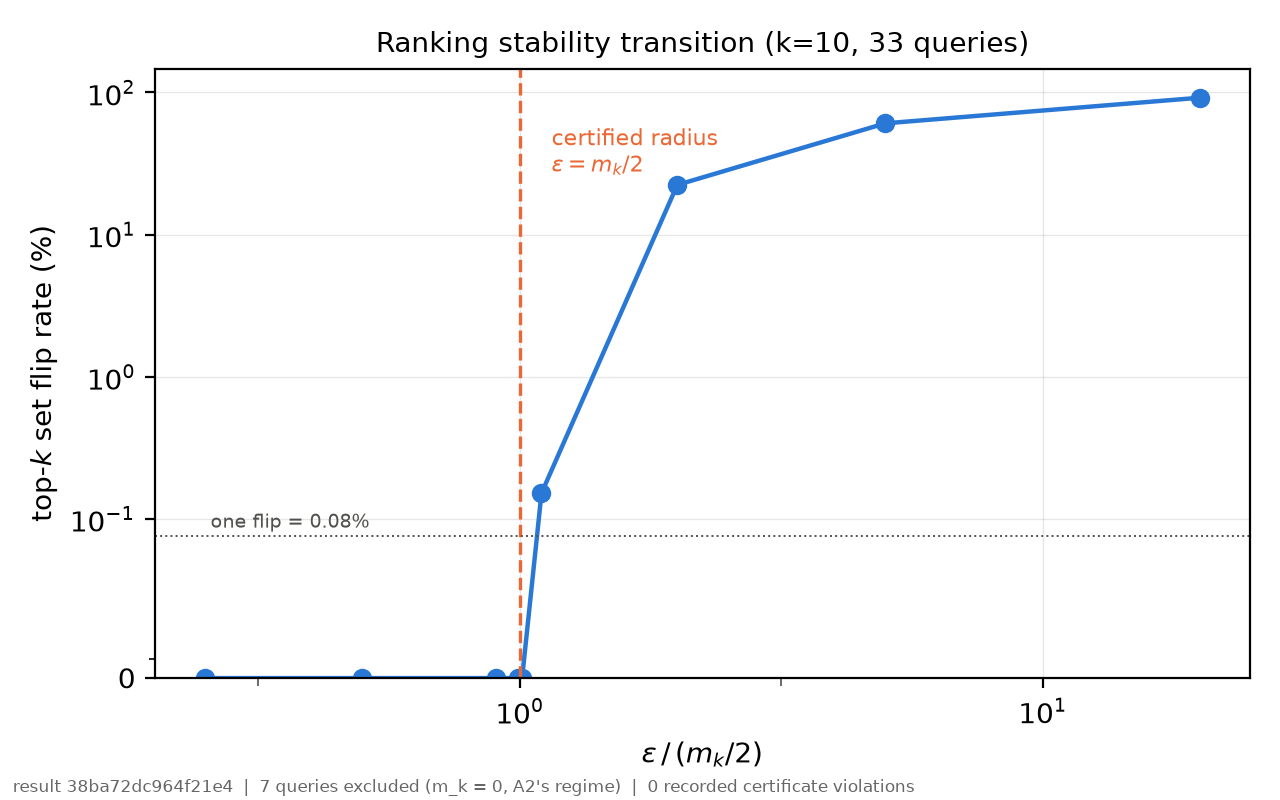
\includegraphics[width=0.78\textwidth]{../figures/fig_transition.png}
\caption{The A1 transition. A non-zero point left of the dashed line would
falsify \S4.4 or the implementation.}
\end{figure}

\section{A2: tie-breaking causes discontinuities}

The claim that tie-break effects are independent of numerical error is earned
structurally. \code{rank\_all\_operators} shares one sorted-score object across
$\pi$, $\pi_{\text{score}}$ and $\pi_{\text{alt}}$, so no arithmetic separates
them and a disagreement admits exactly one cause. The runner verifies this with
bit comparison before reporting anything, and aborts otherwise.

Disagreement concentrates at $k=1$ ($20.0\%$ for $\pi$ against
$\pi_{\text{alt}}$, $16.7\%$ against $\pi_{\text{score}}$), because the leading
document frequently sits in an exact-tie block. That is the decision-level
discontinuity, at the rank where a recommender's output is most visible.

Three corrections belong here.

\begin{enumerate}
\item \textbf{The tie ball is not transitive}, so it is not a partition and
      cannot be used as one. Three objects are provided --- ball, chain and
      clique --- with the chain-inflation ratio $\rho$ relating them
      (\addendum{1}). The dyadic ladder $s_i = i\cdot 2^{-20}$ is the witness.
\item \textbf{The generalised Kendall distance $K^{(p)}$ is a near-metric, not a
      metric}~\cite{fagin2003comparing}. An earlier claim that it satisfies the
      triangle inequality at $p = 1/2$ was wrong; violations were measured at
      every $p$ tested, and the implementation was verified against an
      independently written reference. It is used on bias grounds
      (\addendum{2}).
\item \textbf{\S4.5 does not say which reordering $\pi_{\text{alt}}$ uses.} It is
      pinned to the reversal of $\pi$'s priority. This affects published rates
      and must be stated (\addendum{15}).
\end{enumerate}

\section{\texorpdfstring{\S7.4}{Section 7.4}: near-ties are identified, not constructed}

\S7.4 states that two documents are ``identified such that $|s_A - s_B| \le
\tau$''. The word \emph{identified} is load-bearing.

\begin{finding}\label{find:neartie}
A fine near-tie cannot be manufactured by editing document text. \S2.2 normalises
$\mathrm{tf} = \mathrm{count}/L$, so adding one token changes every term
frequency from $c/L$ to $c/(L+1)$: a \emph{relative} perturbation of $1/(L+1)$
applied to all coordinates at once. A separation of $10^{-9}$ would require a
document of roughly $10^{9}$ tokens.
\end{finding}

What occurs instead is that adjacent gaps are either exactly zero (17--18\% of
pairs) or above roughly $10^{-9}$; the interval between is empty. At fine $\tau$
the near-tie regime therefore \emph{is} the exact-tie regime, and \S7.3's
$m_k \le \tau$ stratum measures the tie-break rather than numerical error ---
A2's regime, not A1's. Conflating them would misattribute the cause
(\addendum{22}).

\section{The scale separation}

\begin{table}[ht]\centering
\caption{Magnitudes measured in this study.}
\label{tab:scales}
\begin{tabular}{lr}
\toprule
quantity & magnitude \\
\midrule
arithmetic noise floor $\eta$      & ${\sim}10^{-16}$ \\
smallest observed score gap        & ${\sim}7\times10^{-10}$ \\
typical adjacent gap               & $10^{-4}$ to $10^{-3}$ \\
corpus-edit perturbation           & $10^{-4}$ to $10^{-1}$ \\
\bottomrule
\end{tabular}
\end{table}

Roughly thirteen orders of magnitude separate the numerical-error regime from the
corpus-perturbation regime, and numerical error never came within six orders of
closing a real gap. A1's bounded perturbations are therefore entirely about
semantic perturbation; floating-point error is not a threat to ranking at any
scale this system operates at. That is a positive result for the numerical design
of \S6, and it is what makes A1 and A2 separable questions rather than two names
for one effect.

\section{Threats to validity}

\paragraph{Configuration dependence.} The noise floor bounds only the
configuration it was measured on. Every experiment records the model digest, and
a run against a different vocabulary or reduction is not covered by that floor.

\paragraph{Finite sampling.} $\eta$ is a maximum over a finite query grid and is
therefore a lower bound on the true worst case. It is reported as measured, with
its grid size, rather than as a proven bound.

\paragraph{Corpus dependence.} The gap distribution shares vary with corpus size,
vocabulary and query; an earlier draft quoted one configuration's table as
canonical and was corrected. What does not vary --- and is enforced by test ---
is that the interval $(0, 10^{-9})$ is empty.

\paragraph{Synthetic data.} The controlled results use a seeded generator.
MovieLens supplies external validity but may not be redistributed, so results on
it are marked non-reproducible-from-repository in their provenance block.

\section{Reproducing every number}

\begin{lstlisting}[language=bash]
python scripts/run_stability_profile.py   --dataset synthetic_small -o reports/
python scripts/run_tie_break_ablations.py --dataset synthetic_small \
       --tau 4.8e-13 -o reports/
python scripts/make_figures.py --reports reports/
python scripts/snapshot.py    # the cross-platform reproducibility digest
\end{lstlisting}

Each runner writes a result envelope whose digest is taken over the payload with
volatile fields stripped, so a rerun on the same data yields the same string and
a published number can be checked by comparing one hexadecimal value. Continuous
integration computes \code{snapshot.py} on Linux, macOS and Windows, at three
optimisation levels and under both backends, and requires every digest to be
identical.

\bibliographystyle{plain}
\bibliography{bibliography}

\end{document}
